%!TEX root = ../main.tex

This chapter will explain the background for the thesis, starting with the introduction of \gls{wrtc}. Then we will look at the use of \gls{wrtc} on mobile devices, look at similar technologies, and current use cases and implementations of \gls{wrtc}. We will last look at Visual Solution's application Virtual Arena for doing collaboration such as audio, video, and application sharing.

\section{Introduction to WebRTC}

\gls{wrtc} is a collection of standards, protocols, and Javascript APIs. The combination of these enables web browsers to do peer-to-peer audio, video and data sharing between browsers. There is no plugin or third-party software required. Real-time communication is now becoming a standard feature in browsers that any web site can use via simple APIs. Delivering functionality such as live audio and video sharing and data exchange requires a lot of new processing capabilities in the browser. We will look at the underlying technologies and protocols of \gls{wrtc}, such as audio and video processing, transportation of media, and security. These technologies are abstracted behind three primary browser APIs:

\newpage
\begin{itemize}
\item MediaStream: capturing audio and video streams
\item RTCPeerConnection: communication of audio and video data
\item RTCDataChannel: communication of arbitrary application data
\end{itemize}

With the above APIs you can: capture media from a camera on your device, do peer discovery, connection negotiations, real-time transportation of media and sharing of arbitrary data. But first of all we look at the working groups behind the development of \gls{wrtc}.

\subsection{Standards and development}
The \gls{wrtc} architecture consists of different standards, covering both protocols and browser APIs:

\begin{itemize}
\item All the different protocols and data formats required to make \gls{wrtc} work is defined by the IETF Working Group \gls{rtcweb}. They are responsible for defining protocols, data formats, security, and all other aspects to enable peer-to-peer communication in the browser.
\item The \gls{wrtc} \gls{w3c} Working Group is responsible for defining the browser APIs.
\end{itemize}

WebRTC is the first open standard to tranport data over \gls{udp} in the browser. However doing this requires a lot more than raw \gls{udp} to do real-time communication, we need media processing and added security layers.

\subsection{Audio and video}
Doing live audio and video sharing requires processing to enhance image quality, doing synchronization, echo cancellation, noise reduction and packet loss concealment\cite{grigorik_high_2013}. On the transmitting end the bitrate must be adjusted to fluctuating bandwidth and latency between clients. On the receiving end the client must decode the streams in real-time and be able to adjust network jitter and latency delays. These are complex problems, but WebRTC includes fully featured engines in the browser, which takes care of all the signal processing for us. All of the processing is done directly by the browser.

\begin{figure}[here]
\centerline{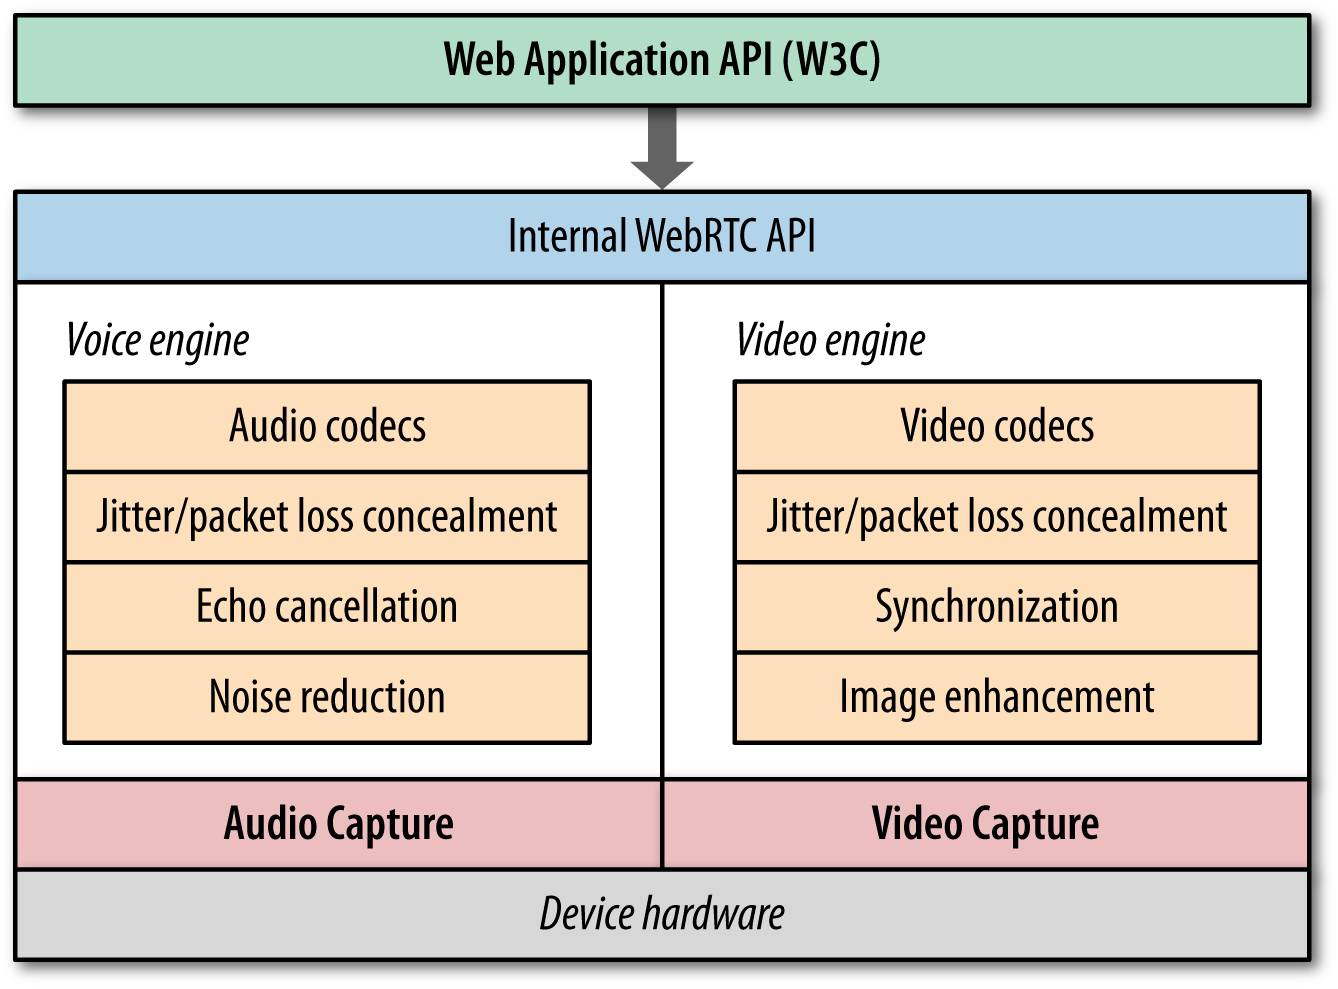
\includegraphics[scale=0.8]{audiovideocapture.png}}
\caption{WebRTC audio and video engines}
\label{fig:audiovideocapture}
\end{figure}

\subsection{Real-time transports}
When it comes to real-time communication, synchronization and low latency is more important than reliability. This is the reason why the \gls{udp} protocol is preferred for doing real-time communication. While \gls{tcp} delivers a reliable communication, there can be delays. If a packet is lost, it is re-requested. The human brain does't handle latency in communication very well, but we are good at filling in the gaps. Therefore we use UDP, which is a connectionless solution. It doesn't check the state of the message. So part of the message could be lost, and we wouldn't know, but the connection would run without delay.

\gls{udp} is the foundation for doing real-time communication, but to meet all the specified requirements of \gls{wrtc}, we need to support a lot of protocols and services on top of that.

\begin{figure}[here]
\centerline{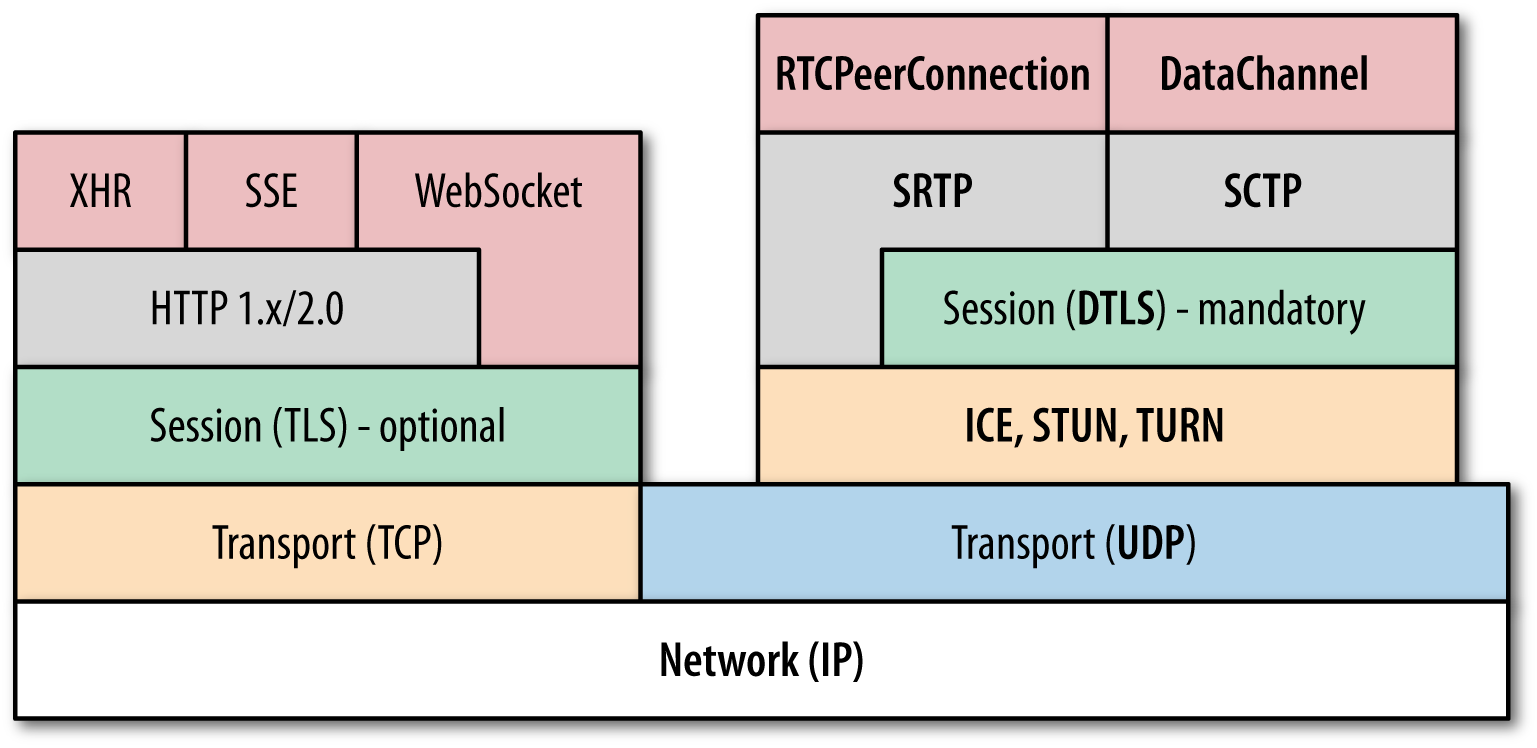
\includegraphics[scale=0.8]{wrtc-protocol-stack.png}}
\caption{WebRTC protocol stack}
\label{fig:wrtc-protocol-stack}
\end{figure}

\gls{ice}, \gls{stun}, and \gls{turn} are needed to establish a connection over \gls{udp} in \gls{wrtc}. Encryption is mandatory and \gls{dtls} is used to secure all transfers between peers. \gls{srtp} and \gls{sctp} are used to multiplex the different streams, provide congestion and flow control, and provide delivery on top of \gls{udp}.

After looking at the underlying technologies of \gls{wrtc} defined as RTCWEB, we will now give an introduction to the drafted browser browser APIs. We are only going to introduce the first two of them, since the third one is not applicable to this project.

\subsection{getUserMedia()}
Acquiring audio and video is done by using JavaScript APIs that enables the browser to acquire audio and video from a physical device such as a webcam or microphone. Incoming streams from remote network peers are also captured and everything is packaged in a MediaStream object. Inside the MediaStream object we have one or more individual tracks that are synchronized with one another. The output can be sent to a local audio or video element, post-processing scripts or remote peers.

The MediaStream object represents a real-time media stream and allows the application to manipulate individual tracks and specify outputs.


The getUserMedia() API allows us to specify a list of mandatory constraints to match the needs of the applicaton:

\lstset{language=Javascript} 
\begin{lstlisting}
var constraints = {
	audio: true,
	video: {
		mandatory: {
			width: { min: 1280 },
			height: { min: 720 },
			frameRate: 30
		},
		optional: []
	}
}

navigator.getUserMedia(constraints, stream, error);
\end{lstlisting}

Once a stream is acquired we can feed them into other APIs such as Web Audio for enabling advanced audio processing. Canvas API for post-processing video frames and WebGL can apply 3D effects on the output stream.

Simplified the getUserMedia() is an API to acquire audio and video streams. The media is automatically optimized, encoded and decoded by the audio and video engines. Then we can display the media locally in an audio or video element in the browser.


\subsection{RTCPeerConnection}
The RTCPeerConnection is responsible for managing the peer-to-peer connection. It uses an \gls{ice} Agent for NAT traversal, keeps track of streams, and triggers renegotiation when required. It provides an API for generating offer and answer.

To be able to understand RTCPeerConnection we need to understand signaling and \gls{ice}.

\subsubsection{Establishing a connection}

\begin{figure}[here]
\centerline{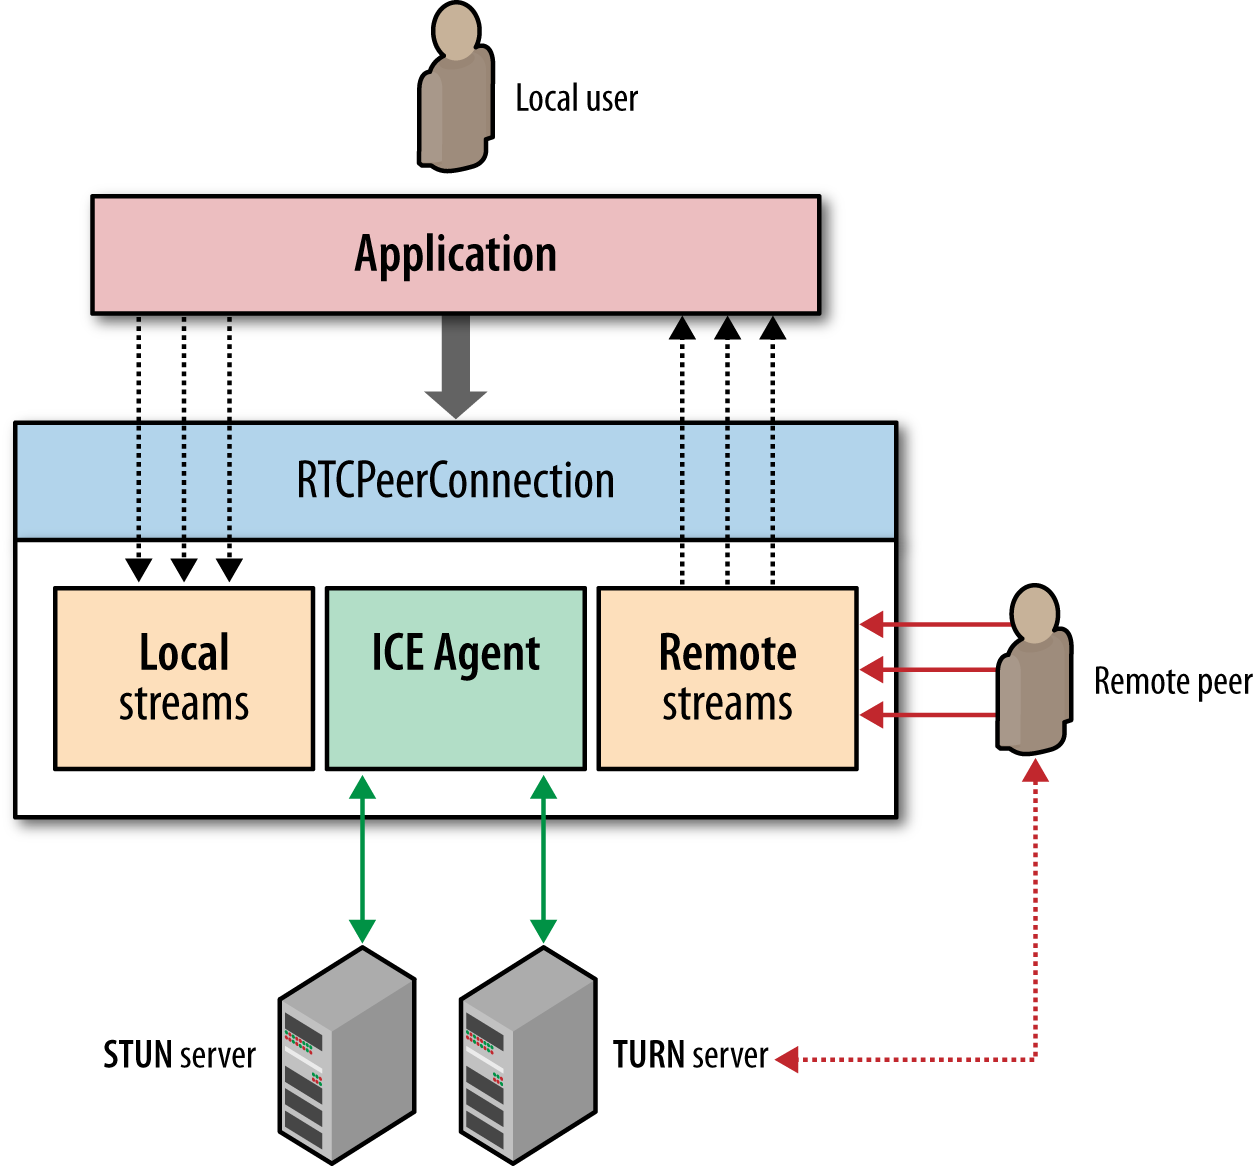
\includegraphics[scale=0.8]{peerconnection.png}}
\caption{RTCPeerConnection API}
\label{fig:rtcpeerconnection}
\end{figure}

\begin{enumerate}
\item Input devices are opened for capture as the media source. This is done using the getUserMedia API.
\item Now we have to signal the other users that we want to connect to them. using RTCPeerConnection we send an \gls{sdp} offer to the other clients, which generates an \gls{sdp} Answer. The \gls{sdp} here includes \gls{ice} candidates,  which allows for firewall traversal.

\begin{figure}[here]
\centerline{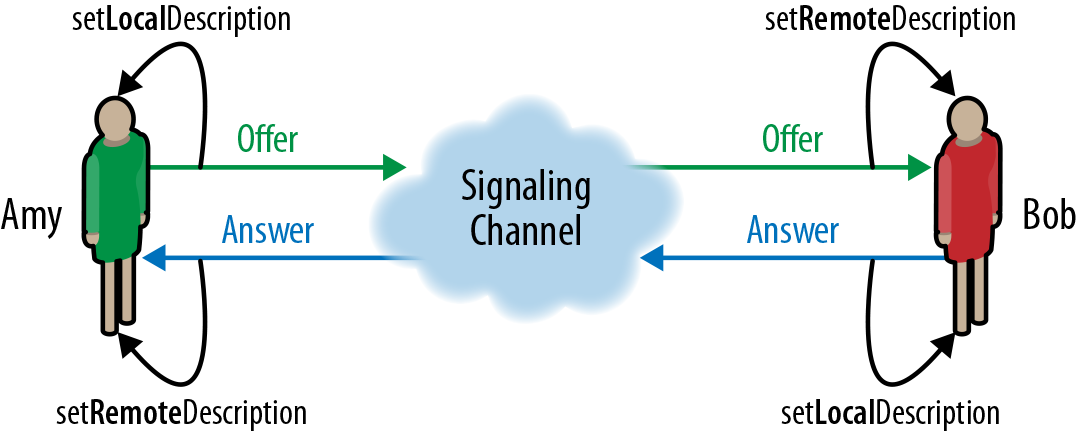
\includegraphics[scale=1.0]{SDPexchange.png}}
\caption{Offer/answer SDP exchange between peers}
\label{fig:sdp-exchange}
\end{figure}

\item Once connection is successful, a \gls{dtls} connection is opened and all the media from input devices are encoded into packets and transmitted using \gls{srtp}-\gls{dtls} streams.
\item At the destination, the packets are decoded and formatted into a MediaStream.
\item The MediaStream is sent to output devices
\end{enumerate}


\subsubsection{Signaling}
While \gls{wrtc} does all the routing and connectivity check for us with the \gls{ice} protocol, we have to do session negotiation ourselves. To do this we must extend an offer to the receiving peer and we need an answer in return. Choice of signaling application is up to us. The \gls{wrtc} standard does not define a signaling protocol, but the key information that needs to be exchanged is the \gls{sdp}, which specifies the necessary transport and media configuration information necessary to establish a connection. This approach is outlined by \gls{jsep}. Assuming we have a shared signaling channel, we can initiate a \gls{wrtc} connection.


\begin{lstlisting}
var signalingChannel = new SignalingChannel();
var pc = new RTCPeerConnection({});

navigator.getUserMedia(constraints, onStream, error);

function onStream(stream) {
  pc.addstream(stream);

  pc.createOffer(function(offer) {
    pc.setLocalDescription(offer);
    signalingChannel.send(offer.sdp);
  });
}
\end{lstlisting}


\subsubsection{SDP}
\gls{wrtc} uses a \gls{sdp} to describe the parameters of a connection. It represents a list of properties describing the connection, ICE candidates, \gls{dtls} parameters, types of media, codecs, bandwidth, \gls{ssrc}s and other metadata information\footnote{http://tools.ietf.org/id/draft-nandakumar-rtcweb-sdp-01.html}.



Here is some of the information that is generated after a call createOffer() has generated the \gls{sdp} description:

\begin{lstlisting}[frame=single]
...snip...
m=audio 1 RTP/SAVPF 111 103 104 0 8 106 105 13 126
c=IN IP4 0.0.0.0
a=rtcp:1 IN IP4 0.0.0.0
a=ice-ufrag:fAYfQM/iWMQPqiHs
a=ice-pwd:pgbuPPRdpKq+obC0lyRxVDe/
a=extmap:1 urn:ietf:params:rtp-hdrext:ssrc-audio-level
a=rtpmap:111 opus/48000/2
a=maxptime:60
a=ssrc:2209464108 cname:7oIEPieg3XZzHJdN
a=ssrc:2209464108 mslabel:uWu6kVvHhYbbkOtNalf5E2LFgjx4cpGMhnfo
a=ssrc:2209464108 label:2b626a18-c54c-4c1b-9f42-03519a9b63f2
m=video 1 RTP/SAVPF 100 116 117
...snip...
\end{lstlisting}


\subsubsection{ICE}
In order to establish a peer-to-peer connection, the peers must be able to send packets to each other. This is easy when you know which ip and port to listen to for incoming messages, but hard when you don't know. Normally there would be firewalls and NAT devices between most peers. In a local environment where there is no firewall, we could establish a connection between two peers by appending the IP and port number to the \gls{sdp}, and forward it to the other peer. What \gls{ice} does is getting around these restrictions by doing connectivity checks and route planning between peers. \gls{ice} gathers all possible addresses it can in address:port and transport triplets\cite{ivov_ice_2013}. \gls{ice} calls these `candidates', and once candidates have been gathered, they are ordered in a list based on priority. Highest priorities are assigned to candidates with the least overhead: those that you get from the device itself, the IP `host' candidates. Next in line are STUN candidates, which are f.ex obtained via \gls{upnp}. Finally the `relayed' candidates that is obtained from TURN servers come. By relaying media through a TURN server, we no longer have a peer-to-peer connection, this is costly and not something we want to do unless there is no other way of connecting to each other.

\subsubsection{Secure communication}
Once we have completed the \gls{sdp} anwers and offers, and traversed NATs, we have come a long way. But \gls{wrtc} require that we encrypt all communication. On top of \gls{udp}, we have \gls{srtp} used for transporting media securely, and \gls{dtls} which is used to negotiate secret keys for encrypting media data. This all taken care of by \gls{wrtc}, and once we have everyting else in place, we are ready to establish peer-to-peer connections.

\subsubsection{Bringing it all together}
To summarize the process of creating a peer-to-peer connection:

\begin{lstlisting}
<video id='local' autoplay></video>
<video id='remote' autoplay></video>

<var ice = {"iceServers": [
    {"url": "stun:stunserver.com:12345"},
    {"url": "turn:turnserver.com", "username": "user", "credential": "pass"}
  ]};

  var signalingChannel = new SignalingChannel();
  var pc = new RTCPeerConnection(ice);

  navigator.getUserMedia({ "audio": true, "video": true }, onStream, logError);

  function onStream(evt) {
    pc.addStream(evt.stream);

    var localVideo = document.getElementById('localVideo');
    localVideo.src = window.URL.createObjectURL(evt.stream);

    pc.createOffer(function(offer) {
      pc.setLocalDescription(offer);
      signalingChannel.send(offer.sdp);
    });
  }

  pc.onicecandidate = function(evt) {
    if (evt.candidate) {
      signalingChannel.send(evt.candidate);
    }
  }

  signalingChannel.onmessage = function(msg) {
    if (msg.candidate) {
      pc.addIceCandidate(msg.candidate);
    }
  }

  pc.onaddstream = function (evt) {
    var remoteVideo = document.getElementById('remoteVideo');
    remoteVideo.src = window.URL.createObjectURL(evt.stream);
  }

  function logError() { ... }
</script>
\end{lstlisting}

\begin{enumerate}
\item{Initialize a shared signaling channel}
\item{Initialize a PeerConnection Object}
\item{Acquire local media streams}
\item{Register local media streams with PeerConnection}
\item{Gather ICE candidates and generate SDP offer describing connection and send to peer via the signaling channel}
\item{Register remote ICE candidates and initiate connection}
\item{Receive remote media stream}
\end{enumerate} 


\subsection{Summary}
We have now looked at the underlying aspects of \gls{wrtc} and the subsequent browser APIs. We know that there are two different working groups: IETF working on the protocols and W3C working on the browser APIs. We also know how to initiate a simple peer-to-peer connection. In the next chapter we will look at some of the challenges of utilizing \gls{wrtc} on a mobile device.

\newpage
\section{Mobile devices}
%!TEX root = ../main.tex

The use of mobile broadband for accessing the Internet via tablets and smartphones has increased rapidly as a result of high speed mobile networks becoming more available such as 3G and 4G. The web browser on these devices are becoming more and more similar in capabilities to their desktop versions. It is possible to run \gls{wrtc} applications in some of them, and these features will become more available with time. This section is going to look at the use of \gls{wrtc} in mobile devices. We start by looking at some of the issues we have to deal with when working with mobile devices, then we will look at performance and quality metrics derived from current research.

\subsection{Network performance}
It is feasible to run \gls{wrtc} applications on mobile devices. However, battery consumption,  persistent connectivity, and quality performance remain a big challenge. A lot of work is being done in radio technologies, but the most important factor is how the applications, protocols, and API's are designed\cite{isomaki2012considerations}. First we will look at some of the performance issues of serving wireless video.

The most used and relevant networks are Wi-Fi, WiMAX, and the different telecommunication networks. Serving wireless video is a significant challenge for already-stressed cellular data networks\cite{erman2011over}. Video traffic requires high bandwidth, imposes latency and packet loss. The key is to deliver video as high in quality as the network supports. By looking at a study testing video and audio quality on two differenet WiMAX networks\cite{fund2013performance}, we can see variations of performance in two different locations.

\pagebreak
\begin{figure}[here]
\centerline{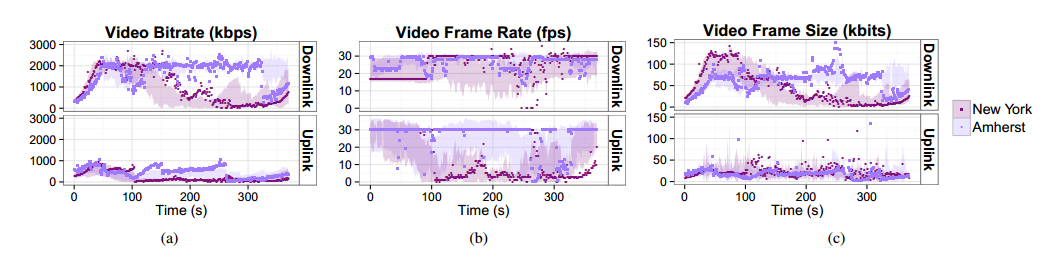
\includegraphics[scale=0.4]{mobile-video-metrics.png}}
\caption{WebRTC video performance. For each plot, the shaded area shows one standard deviation above and below the mean, while the
points give values for a representative trial. These values are presented from the perspective of the mobile, WiMAX-connected peer.
}
\label{fig:mobile-video-metrics}
\end{figure}

\gls{wrtc} adapts to changing link conditions by estimating the available sent bandwidth and passing this estimate to the encoder as a target bitrate. Figure \ref{fig:mobile-video-metrics} show key metrics of video and audio quality for a \gls{wrtc} session sustained over a WiMAX link in two different locations. There is a dramatic difference in performance between the two locations, with the suburban setting always outperforming the urban setting. The uplink stream has significantly worse video performance, this is probably due to the asymmetry of the celullar link, only 25\% of radio resources are allocated to the uplink\cite{fund2013performance}. A result of this is a reduced frame rate, this is unfortunate since mobile users are often walking, which makes the video feed have a high motion content.

\pagebreak
\begin{figure}[here]
\centerline{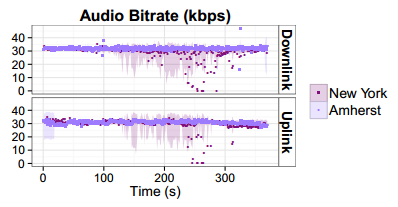
\includegraphics[scale=0.4]{mobile-audio-metrics.png}}
\caption{WebRTC audio performance shown as representative values
(points) and a range of one standard deviation above and below the
mean (shaded area).}
\label{fig:mobile-audio-metrics}
\end{figure}

An important thing to mention is that video quality is not that important when it comes to communication, the audio quality is of much more value\cite{fund2013performance}. We can observe from Figure \ref{fig:mobile-audio-metrics} that the audio bitrate is mostly consistent, degrading only in extremely poor channel quality. The biggest problem here as seen in Table \ref{tbl:wrtc-packet-loss} is that the packet loss is quite high on the uplink for audio in the urban environment. This is because the quality is not reduced to keep the audio signal clear. This could be somewhat fixed by retransmission of the packets, but this will again increse latency.
\\
\begin{table}[here]
\centerline{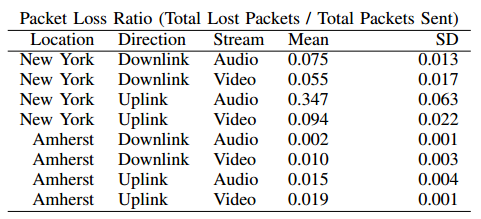
\includegraphics[scale=0.4]{wrtc-packet-loss}}
\caption{Packet loss ratio for a WebRTC session.}
\label{tbl:wrtc-packet-loss}
\end{table}

\subsection{Connectivity}
Another concern is persistent connectivity. For an app to be reachable for incoming connections, it needs some kind of persistant communication channel. Most cellular networks have a firewall preventing incoming TCP connections\cite{isomaki2012considerations}. To keep a TCP connection alive, the application needs to send some kind of keep-alive packets with a high enough frequency to avoid a connection timeout. Problem with keeping a connection open all the time is that is that device's radio will consume a lot battery. Therefore, the keep-alive packets should only be sent infrequently.

\subsection{Summary}
Most of the performance issues is handled by the underlying technologies of \gls{wrtc}, which actually is pretty good at adapting bandwidth usage in variable network conditions, but it is important to be aware of these problems when developing applications. The effect that a mobile users uplink is much worse than its downlink has great impact on a user's perception of the connection. However, the most important factor for us to consider is how we will do the signaling with a mobile device, since we can't keep a connection open all the time, as that would drain the battery.

\newpage
\section{Related technologies}
There are a lot of implementations of real-time communications out on the market today. Let's take a look at similar technologies\cite{lopez_fernandez_catalysing_2013} that is in direct competition with \gls{wrtc}:

\subsection{Real-time communications}
For doing real-time communications we have commercial services such as Skype, Tokbox, and Google Hangout. 

Skype is definately the biggest one in this category. Skype utilizes peer-to-peer technology by leveraging all of the available resources in a network, this is probably why they can manage free communications. Using centralized resources is very costly. Skype has very successfully developed a video collaborations system utilizing peer-to-peer technology, but the quality depends on the users available resources. This is the same with the current networking model of \gls{wrtc}.

\subsection{Live broadcasting}
Services that does live broadcasting such as Ustream, Twitch, and Google Chromecast are also in competition with \gls{wrtc}. 

A lot of e-commerce sites are looking to integrate \gls{wrtc} as part of their customer service experience. Today it is normal to have live text chat, but with \gls{wrtc} it is easy to integrate video support as well.

In addition we have vendors providing technologies at different layers of the protocol stack such as Microsoft's Lync and Apple's FaceTime. It is also worth to mention common open source services like Asterisk\footnote{Telephony switching services} that are heavily used in commercial software. Asterisk has recently increased their signaling services to support \gls{wrtc} as well.

These companies have made significant investments to build their services, and with the introduction of \gls{wrtc} these companies are both threatened by competing businesses, but the tehcnology also opens up for new opportunities.

There exixst two public projects for doing server-side processing of media namely Tokbox and Lynckia. Righ now these services are limited to interact with other \gls{wrtc} endpoints. There is no interoperability with non \gls{wrtc} clients.

Missing technologies in \gls{wrtc} that we can find in other services, are PUSH capabilities, interop with other legacy systems such as SIP, more flexible group conversation architecture, advanced media sharing capabilities. These would require server-side capability.

\newpage
\section{Current implementations}
%!TEX root = ../main.tex

There are some quite popular implementations of \gls{wrtc} today, although very few of these use \gls{wrtc} exclusively, we will mention a couple of the most popular ones, along with some platforms for simplifying \gls{wrtc}.

\subsection{Browsers}
Google's desktop and android versions of Chrome incorporates \gls{wrtc}, as does Firefox. \gls{wrtc} support on Opera is on the way. There is still uncertainty about when Internet Explorer will add support. Google and Mozilla has displayed interoperability between Chrome and Firefox. This is necessary to achieve transparency regarding the browser being used, therefore preventing the use of a particular browser. 

\subsection{Hangout}
Google's Hangout\footnote{http://www.google.com/hangouts/} is competing with Skype in the desktop videoconferencing space. Parts of the \gls{wrtc} stack is implemented in Hangout's code base, but Hangout is not a pure \gls{wrtc} implementation yet, simply because it needs to work on every browser, therefore it is packaged in a browser extension, but the underlying works relies heavily on \gls{wrtc} technologies.

\subsection{Chromecast}
Google's Chromecast\footnote{http://www.google.com/intl/en/chrome/devices/chromecast/index.html} uses \gls{wrtc} as well, but in a different way than Hangout. It is only used for one-way streaming from you device to a TV. Other services in the live broadcasting space such as Twitch\footnote{http://www.twitch.tv/} could be seeing competetion from \gls{wrtc} in the near future.

\subsection{WeCam and API platforms}
The app WeCam\footnote{http://wecamchat.com/} let's you video chat with your Twitter, Google+, and Facebook friends. It uses an API platform called OpenTok that simplifies much of the \gls{wrtc} setup, such as signaling. By leveraging platforms you suddenly get access to a lot more features on top of \gls{wrtc}, but these platforms cost money. Then again they add important functionality that's missing from \gls{wrtc}, such as being able to do processing of media. Two examples of public projects for doing server-side processing of media are Tokbox and Lynckia. Right now these services are limited to interact with other \gls{wrtc} endpoints and there are no interoperability with non-\gls{wrtc} clients. Other missing technologies in \gls{wrtc} that we can find in related services are PUSH capabilities, interoperability with legacy systems such as SIP, more flexible group conversation architecture and advanced media sharing capabilities. All of these currently require some sort of server-side architecture.

\subsection*{Summary}
\gls{wrtc} is definately on the right path to becoming big, as it's being utilized in a couple of very popular applications, but right now it's missing some key features to become a permament solution for companies. It currently acts more like a tool to simplify much of the underlying aspects of doing real-time media, you have to take care of the rest yourself. One of the big things that's missing are being able to do processing of media, however upcoming companies sell their services on top of \gls{wrtc} to allow for these features.

\newpage
\section{Virtual Arena}
%
This section will first introduce the company Visual Solutions\footnote{http://www.bbvisuals.com/} who provided the practical problem. Secondly I will give a quick overview of how the application Virtual Arena works by describing its underlying architecture, then I will look at how the enterprise firewall works, and lastly look some of the security concerns that occur when a enterprise collaboration system has to access the public internet.

\section{Visual Solutions}
Visual Solutions is a Norwegian company in the BB Visual Group\footnote{http://www.bbvisualgroup.com/}. Their primary business is within the integration of operations for the oil and gas industry. They create solutions enabling collaboration across organisation units and geographic locations. One of their applications Virtual Arena\cite{solutions_b2_virtual_2014}, which from now on will be referred to as VA, is a powerful and interactive tool that allows for high-performance application sharing, with audio and video communication from a 3D shared scene\ref{fig:?}. VA supports many-to-many collaborative scenarios by utilizing a media server which will be described in the next section. 

\section{Virtual Arena}
VA is the application that Visual Solutions has created for doing visual collaboration\cite{VirtualArena} over IP. The architecture of VA is visualized in Figure\ref{?}. The application uses a media server that serves multiple purposes. It acts as a \gls{mcu}, applies mitigation strategies for scenarios with limited bandwidth, and also sharing of applicaton data. Mitigation strategies can f.ex be reducing the video bitrate to adjust adapt for a poor connection. The media server works together with a router for distributing the streams. By utilizing a media server VA can support a lot incoming and outgoing streams. A client can subscribe to multiple streams of audio/video and applications. It manages these connections using a tree structure, but this is an advanced topic that I won't go into detail about. In the next subsections the different parts of the architecture\ref{?} will be described with the necessary information required to understand the practical problem this thesis will try to solve. 
\\
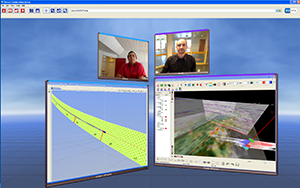
\includegraphics[scale=0.6]{virtualarena.png}
\\
\\

\subsection{Signaling}
VA has a proprietary way of doing signaling over RTCP. RTCP is control protocol for RTC. This is where the clients send messages to the media server describing which streams they want to subscribe to. Communication between peers and the media server is done by opening up ports in the firewall to listen for incoming TCP and UDP connections. These ports are preconfigured for the application. The media server can receive incoming streams and route it to all peers connected. The streams are identified using a SSRC, which is defined in the header packets of the RTP streams.

\subsection{Transport layer}
VA uses raw RTP stream over UDP. This is basically the most standard protocol used for transmitting real-time data in enterprise communication systems\cite{}.

\subsection{Media}
VA uses free and open source codecs for audio and video. It uses Speex for audio, and Theora for video. These are not the most commonly used codec, as the g.711 for audio and H.264 for video are the most common ones. Even though H.264 is licensed by Ericsson, it offers the added benefits of hardware acceleration in a lot of graphic cards, and is also one of the best codecs for real-time streaming as of now\cite{source}.

%%are common in, but h.264 g.711 standard in ims systems%%

\subsection{Security}
VA only uses raw UDP streams because nothing more is needed. It operates in a closed business environement, so transport level encryption is not needed, because unidentified peers are not allowed inside the network anyways. The enterprise firewall has very strict policys, only allowing certain kinds of traffic.?????

\subsection*{Summary}
VA operates like a typical enterprise comunication system. CODEC?? 

\newpage
\section{Summary}
\gls{wrtc} brings a lot of new technologies to the table. It is an effective tool that can be used to quickly create real-time communication applications, with the added advantages of being platform independant. With the new APIs we can run a client on any tablet or mobile device that has a web browser with support for the \gls{wrtc} standard. Related technologies developed by Cisco and Microsoft are more complete and are now dominating the communication space, but it's going to be interesting to see if they will loose some markets to smaller companies utilizing \gls{wrtc} in the future. Google has successfully used \gls{wrtc} in their Hangout application and on their Chromecast devices. Probably the biggest problem with \gls{wrtc} right now is that the IETF working group have not agreed on a video codec yet, which is somewhat halting the development. Visual Solutions Virtual Arena is using transport technologies that needs to have added security layers to work with \gls{wrtc} and the media formats needs to be transcoded with the appropriate codecs. Also the signaling and routing needs to be enhanced to make Virtual Arena work with \gls{wrtc}. In the next chapter we will go further into the problems of integrating \gls{wrtc} with Virtual Arena.